\section{PDE Discretization}
Multidimensional topological optimization problems often involve the use of partial differential equations (PDEs) which model the physical properties of the materials involved. Most of these PDEs cannot be uniquely solved analytically, so we turn to numerical methods in order to approximate their solutions. The first step in many of these methods is to discretize our domain; that is, we want to choose some scheme to divide our continuous domain into a finite number of pieces over which we will apply a particular method to approximate solutions to the PDE.

In the SIMP method, the Finite Volume Method is used to discretize and approximate solutions to the heat equation for our heat generating medium. We will introduce the Heat Equation and then proceed to give an overview of the Finite Volume Method.
\subsection{The Heat Equation}
Consider a stationary object of that has heat flowing between its interior regions. The temperature at any point in the interior of the object will depend on the spatial position chosen as well as the time we measure the temperature at that point. Therefore, the temperature ($T$) at any point in such an object is a function of both space ($\vec{x}$) and time ($t$) coordinates: $T(\vec{x},t)$.
Physical principles demand that such a temperature function must satisfy the equation
\begin{equation}
	\frac{\partial T}{\partial t}=\nabla\cdot\left(k(\vec{x})\nabla T\right)\label{eqn:HeatEq},
\end{equation}
where $\nabla$ is the gradient operator (also known as ``del'') and the function $k$ represents the thermal diffusivity at a point in our object.

Equation (\ref{eqn:HeatEq}) is commonly referred to as the Heat or Diffusion Equation. If we were to have a constant thermal diffusivity throughout our object, it would be possible to analytically find a solution to this partial differential equation. However, as in the problems of interest throughout this paper, when $k$ is not constant we must turn to numerical methods to find approximate solutions for the function $T$.

\subsection{The Finite Volume Method}

For our numerical approximations of PDEs in this paper, we used the Finite Volume Method (FVM).

As with any other numerical method to solve PDEs, we must first discretize our domain by creating some sort of mesh. One major advantage of the Finite Volume Method is that we have a great amount of freedom in choosing our mesh. In FVM the domain can be discretized into a mesh of arbitrary polygons, but we chose uniform squares in our work to simplify the resulting calculations.

\subsubsection{The Finite Volume Method in Two-Dimensions}

\begin{figure}
	\centering
	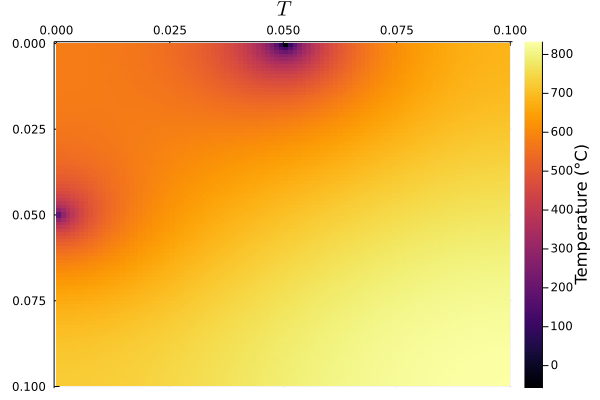
\includegraphics[width=0.8\textwidth]{Chapter_I_Background/Images/T-Heatmap_2_Heatsinks.png}
	\caption[Heatmap Example]{Heatmap for a \SI{0.1}{\meter} $\times$ \SI{0.1}{\meter} object with uniform heat generation and 2 heatsinks on its north and west boundaries. This map was produced via the Finite Volume Method using $100\times 100$ uniform control volumes.}
\end{figure}